% !TeX root = RJwrapper.tex


  \title{\pkg{FuzzySimRes}: Epistemic Bootstrap -- the Efficient Tool for Statistical Inference Based on Imprecise Data}
  \author{by Maciej Romaniuk, Przemys{\l}aw Grzegorzewski, Abbas Parchami}
  
  \maketitle
  
  \begin{abstract}
  The classical Efron's bootstrap is widely used in many areas of statistical inference, including imprecise data.
  In our new package \CRANpkg{FuzzySimRes} we adapted the bootstrap methodology to the epistemic fuzzy data, i.e. fuzzy perceptions of the usual real-valued random variables.
  The epistemic bootstrap algorithms deliver real-valued samples generated randomly from the initial fuzzy sample.
  Then, these samples can be utilized directly in various statistical procedures.
  Moreover, we implemented a practically oriented simulation procedure to generate synthetic fuzzy samples and provided a real-life epistemic dataset ready to use for various techniques of statistical analysis.
  Some examples of their applications, together with the comparisons of the epistemic bootstrap algorithms and the respective benchmarks, are also discussed.
  \end{abstract}


%%%%%%%%%%%%%%%%%%%%%


\section{Introduction} 
\label{intro}

Efron's bootstrap \citep{EfroTibs93} is a simple but very powerful tool. This useful resampling method is successfully applied in statistical inference, including estimation, hypotheses testing, and other data analysis techniques, e.g., \cite{davison_hinkley_1997,ISLR,romaniuk2019}.

In our package \pkg{FuzzySimRes} we adapted the classical bootstrap algorithm to a special kind of imprecise data, i.e. the epistemic random fuzzy numbers (see \cite{Couso2014}), which might be treated as fuzzy perceptions of the usual real-valued random variables.
This way, a special resampling methodology, known as the epistemic bootstrap, can be introduced \citep{grzegorzewski2021,10.1007/978-3-031-08974-9_39,pgmr2022}.
Following the suggested methods we can generate random real-valued samples based on the initial fuzzy sample.
Such a ``change of a viewpoint'' from the ``fuzzy world'' to its ``clear'' (i.e. real-value) counterpart can be a very useful and important tool.
This allows all commonly used classical statistical methods (developed for real-valued samples), including statistical tests, estimation procedures, etc., to be directly and easily adapted to fuzzy epistemic samples.





Please note that statistical inference for the fuzzy data is usually underdeveloped, poses some problems, and leads to discussions about the intuitions, solutions, etc. (e.g., concerning the different approaches to the p-value).

We provide some useful functions in our package \pkg{FuzzySimRes}.
They are related to a practically oriented simulation of various types of fuzzy numbers (FNs), the epistemic bootstrap itself, and its applications related to the estimation of important statistical measures of the initial sample, and the one- and two-sample statistical tests.
Additionally, we provide the real-life dataset of the epistemic FNs, which can be useful in comparing various approaches to fuzzy statistical inference.
Based on the two general epistemic bootstrap functions, users of \pkg{FuzzySimRes} can build their own ``epistemic bootstrap statistical tools'' to fit their purposes (e.g., the necessity of using tests other than the Kolmogorov-Smirnov one).

In the following, we briefly compare \pkg{FuzzySimRes} package with other existing ones and introduce a necessary notation.
Then, the functions implemented in the package are illustrated with the respective examples.
Finally, the outcomes of these functions are compared taking into account some benchmarks for different statistical problems using both the synthetic and real-life data. 


%%%%%%%%%%%%%%%%%%%%%

  
\subsection{A brief review of related packages}

There are some packages related to fuzzy numbers and their statistical analysis.
Firstly, we should mention \CRANpkg{FuzzyNumbers} \citep{FuzzyNumbersMan}.
This library aims to provide S4 classes and methods for FNs.
They can be used to construct different types of FNs (e.g., triangular or trapezoidal ones), compute arithmetic operators for fuzzy values, calculate their approximations, and find different characteristics of FNs (like the possibility and necessity values, expected interval, ambiguity, membership functions among many others) for arbitrary FNs or some of their special types, etc.
Notably, our package \pkg{FuzzySimRes} uses S4 objects describing FNs derived from this package.
However, there are no special functions devoted to simulations or resampling methods in \pkg{FuzzyNumbers} package.
Therefore, it can be seen as a kind of ``foundation'' to deal with FNs.

The next package, \CRANpkg{FuzzySTs} \citep{FuzzySTsMan} is a collection of various statistical tools, like fuzzification methods, numerical estimations of fuzzy statistical measures and bootstrap distribution of the likelihood ratio, testing hypotheses by fuzzy confidence intervals and estimation of the fuzzy p-values for epistemic fuzzy data.
These approaches are related to fuzzy notions, like fuzzy p-values, resulting in the strictly fuzzy output \citep{Berkachy2019}.

And \CRANpkg{SAFD} \citep{Trutschnig2013} package joins two kinds of functions.
Similarly to \pkg{FuzzyNumbers}, it provides basic operations on FNs (like the sum, mean, etc.), but it also contains some strictly statistical functions.
They allow us to simulate FNs and perform bootstrap tests for the equality of the means.
As for the simulation function, this is an implementation of the second procedure described by \cite{GONZALEZRODRIGUEZ2009642}, where a respective basis is perturbated stochastically to generate
a new polygonal fuzzy number.
There are important theoretical and practical differences \citep{FRV} between this approach and the one applied in \pkg{FuzzySimRes} package.
The statistical tests in \pkg{SAFD} library are exclusively based on the classical bootstrap as described by \cite{COLUBI2009344,Montenegro2004}.

On the other hand, \CRANpkg{Sim.PLFN} \citep{SimPLFNMan} can be seen as a kind of ``ancestor'' of our package.
It allows only to simulation of some kinds of FNs some kinds of FNs, especially so-called piecewise linear FNs \citep{COROIANU201326}, and calculates a few basic operators (like the sum, mean, and variance) for them.

Another package, \CRANpkg{FuzzyStatTra} \citep{FuzzyStatTraMan}, also provides basic statistical functions for FNs like calculation of the mean and medians, indexes, and various distance measures.
Some simulation procedures are also included there, but they are intended for special cases of dependent and independent components described by \cite{7295579}.
Therefore, they can not be considered as ``multi-purpose'' generation functions when the probability distributions are selected by the user.

We should also mention our previous package, \CRANpkg{FuzzyResampling} \citep{FuzzyResampling} that provides various resampling algorithms other than the classical bootstrap \citep{fuzzyResamplingArt}.
The main aim of these approaches is to overcome a problem with repetition of a few distinct values (which is commonly seen in the case of the Efron's bootstrap) and to create FNs, which are ``similar'' (in the sense of some characteristics of FNs) but not ``the same'' as values from the initial sample \citep{grzegorzewski_amcs2020,romaniuk_hryniewicz,GrzegorzewskiRom2021}.
Additionally, the tests for the means related to the approach presented by \cite{LUBIANO2016918} but based on these new resampling methods are also provided.

Nevertheless, \pkg{FuzzySimRes} has some unique features.
Firstly, it adds very useful simulation functions (as its acronym -- Fuzzy Simulations and Resampling -- suggests) to complete \pkg{FuzzyNumbers} in this field.
These procedures are very intuitive and practically oriented as noted by \cite{FRV} (contrary to, e.g., \pkg{SAFD} that adds some random noise without keeping track of important characteristics of the input FNs).
Secondly, the so-called epistemic bootstrap is implemented there.
Apart from ready-to-use general epistemic bootstrap functions, special procedures are provided for the estimation of parameters of the underlying statistical model, together with an interface that can be used with various classical statistical tests.
The epistemic bootstrap is a relatively new idea and the respective algorithms were not implemented in other publicly available software packages (including R itself).
It should be noted, that this approach is completely different when compared with the ontic-oriented resampling procedures from \pkg{FuzzyResampling} that can be seen as a ``generalization'' of the classical bootstrap procedure \citep{grzegorzewski_amcs2020,GrzegorzewskiRom2021}.


%%%%%%%%%%%%%%%%%%%%%%%%%%%%%%%%%%%%%%%%%%%%%%%%%%%


\subsection{Epistemic fuzzy numbers}

In the following, we recall some basic concepts and notations concerning fuzzy numbers. For a more detailed introduction, we refer the reader to, e.g., \cite{ban_coroianu_pg}.

A \textbf{fuzzy number} (abbreviated further as FN) is an imprecise value characterized by a mapping $\tilde{A}:\mathbb{R}\to [0,1]$ (a \textbf{membership function}), such that its $\alpha$-cut defined by
\begin{equation}
\tilde{A}_{\alpha}=\begin{cases}
\{x\in\mathbb{R}:\tilde{A}(x)\geqslant\alpha\} & \text{if}\quad \alpha\in (0,1], \\
cl\{x\in\mathbb{R}:\tilde{A}(x)>0\} & \text{if}\quad \alpha=0,
\end{cases} \label{eq_acut}
\end{equation}
is a nonempty compact interval for each $\alpha\in [0,1]$. Operator $cl$ in \eqref{eq_acut} denotes the closure. Every FN is completely characterized both by its membership function $\tilde{A}(x)$ and a family of $\alpha$-cuts $\{\tilde{A}_{\alpha}\}_{\alpha\in [0,1]}$. There are two special $\alpha$-cuts: the \textbf{core} $\tilde{A}_1=\mathrm{core}(\tilde{A})$, which contains all values fully compatible with the concept described by $\tilde{A}$, and  the \textbf{support} $\tilde{A}_0=\mathrm{supp}(\tilde{A})$ on real line, for which values are compatible to some extent with the concept modeled by $\tilde{A}$. A family of all FNs will be denoted by~$\mathbb{F}(\mathbb{R})$.

There are many possible shapes of the membership functions.
A special family of the \textbf{LR-fuzzy numbers} is defined by
\begin{equation} 
\tilde{A}(x)=
\begin{cases}
 0 & \text{if}\quad x < a_1,  \\
 L \left( \frac{x-a_1}{a_2 - a_1}\right) & \text{if}\quad a_1 \leqslant x < a_2 ,  \\
 1 & \text{if}\quad a_2 \leqslant x < a_3 , \\
 R \left( \frac{a_4 - x}{a_4 - a_3}\right) & \text{if}\quad a_3 \leqslant x < a_4 , \\
 0 & \text{if}\quad x \geqslant a_4,  
\end{cases}
\label{eq:LFfn}
\end{equation} 
where $L, R: [0,1] \rightarrow [0,1]$ are continuous and strictly increasing function such that $L(0)=R(0)=0$ and $L(1)=R(1)=1$, and $a_1,a_2,a_3,a_4\in\mathbb{R}$, where $a_1\leqslant a_2\leqslant a_3\leqslant a_4$. If $L$ and $R$ are linear functions, i.e. $L \left( \frac{x-a_1}{a_2 - a_1}\right) = \frac{x-a_1}{a_2 - a_1}$ and $R \left( \frac{a_4 - x}{a_4 - a_3}\right) = \frac{a_4 - x}{a_4 - a_3}$, we get a \textbf{trapezoidal fuzzy number} (denoted further on as TPFN). Moreover, if $a_2=a_3$ then we have a \textbf{triangular fuzzy number} (abbreviated as TRFN).
In these two cases, we can simply write $A=(a_1, a_2, a_3, a_4)$ (for TPFN) or $A = (a_1, a_2, a_4)$ (for TRFN) to fully describe such FNs.

Another type of the LR-fuzzy number is known as the \textbf{$k$-knot piecewise linear fuzzy number} \citep{Coroianu2019} (or polygonal fuzzy number, see \cite{Baez2012}, abbreviated further as PLFN), which is suitable especially in an approximation of more complex FNs.
In this case, $L$ and $R$ functions are polygons consisting of $k\in\mathbb{N}$ segments.

Fuzzy numbers are used to model the results of various experiments that cannot be precisely described, qualified, or measured.
But in many cases, we have to draw conclusions and make decisions based on data whose uncertainty comes both from randomness (which classical statistics copes with) and lack of precision (for which the fuzzy set theory is perfect for modeling). To model such data one can use \textbf{fuzzy random variables}, known also as \textbf{random fuzzy numbers} \citep{FRV}.

It should be noted here that we can look at fuzzy random variables from two different perspectives: \textbf{ontic} or \textbf{epistemic} (e.g. \cite{Couso2014}). The first concerns data that appear to be essentially fuzzy in value, while the second refers to situations where, although precise (accurate) data values exist, they are imprecisely observed (e.g. due to imperfections in measuring devices, inaccuracies caused by people performing the measurements, or how results are reported), so their true actual values remain unknown. This second kind of imprecision is widespread in real-life problems met in engineering, science, and other applications, so further on we limit our attention only to epistemic data.

Following the definition by \cite{Kwakernaak} and \cite{Kruse1982} a fuzzy random variable $\widetilde{X}$ can be considered as a \textit{fuzzy perception} of the unknown random variable $X$, called the \textit{original} of $\widetilde{X}$. More precisely, given a probability space $(\Omega,\mathcal{F},P)$, a mapping $X:\Omega \to\mathbb{F}(\mathbb{R})$ is said to be a fuzzy random variable (f.r.v.) if for each $\alpha\in [0,1]$ $(\inf X_\alpha):\Omega\to\mathbb{R}$ and $(\sup X_\alpha):\Omega\to\mathbb{R}$ are real-valued random variables on $(\Omega,\mathcal{F},P)$. Similarly, a \textbf{fuzzy random sample} $\widetilde{X}_1,\ldots,\widetilde{X}_n$ is a fuzzy perception of a random sample $X_1,\ldots,X_n$ of the usual real-valued random variables. For more details, we refer the reader to \cite{Kwakernaak,Kruse1982}.

\subsection{Epistemic vs classical bootstrap}

There are important differences between the classical Efron's bootstrap \citep{EfroTibs93} and its epistemic counterpart \citep{grzegorzewski2021,pgmr2022,PGMR2024AMS}.
In the classical bootstrap approach, the initial sample is then directly resampled.
Therefore, in the case of fuzzy input, the output also consists of the same FNs as in the primary sample (with possible repetitions or omitting some of them).
This procedure can be very useful in statistical inference (see, e.g., \citep{gil,LUBIANO2016918,Montenegro2004}) but the respective statistical tests (or other statistical procedures like the estimation) have to be specially developed for fuzzy-valued samples.
Therefore, there is a need to construct ``almost completely new'' statistical solutions taking into account various distance measures for fuzzy sets existing in the literature, more complex definitions of the expected value, possible problems with difference operator, etc. \citep{ban_coroianu_pg,HEILPERN199281}.
Resampling procedures existing in \pkg{FuzzyResampling} package can be seen as a kind of generalization of this classical bootstrap (in the same manner as the smoothed bootstrap in the case of real-valued samples).
They aim to preserve some important characteristics of FNs (like the value, ambiguity, etc.) but with an alternation of FNs from the initial sample into ''new'' values occurring in the generated samples \citep{grzegorzewski_amcs2020,GrzegorzewskiRom2021}.
However, we are still obtaining fuzzy-valued outputs for these methods.

On the other hand, in the epistemic bootstrap, a completely real-valued (i.e. ``crisp'') sample is generated from a fuzzy-valued initial sample.
It allows to use of directly highly developed statistical tools for real-valued data (various statistical tests, point or interval estimators, etc.) without the need for transforming them into a ``new fuzzy world''. 
Consequently, knowing statistical tools with suitable good properties, the areas of possible applications of epistemic fuzzy data may substantially expand.
To explain it better, consider the following goodness-of-fit testing problem. In \cite{LUBIANO2016918} and \cite{lubiano2017}, the outcomes of the well-known questionnaire TIMSS-PIRLS 2011 performed by Spanish primary school pupils were considered, while in  \cite{Ramos-Guajardo2019} experts' perceptions about different characteristics of the Gamonedo blue chees were discussed. In both cases, researchers dealt with subjective valuations expressed in natural language, which are inherently imprecise, and therefore modeled using ontic fuzzy sets. Thus, the problems mentioned above required the construction of appropriate statistical tools that would enable inferences to be made based on this type of data.
Meanwhile, the epistemic variants of the classical Kolmogorov-Smirnov and Cramer-von Mises tests were directly used for fuzzy data concerning the lifetimes of street light equipment \citep{Hesamian2013} and electronic circuit thickness \citep{FARAZ20102684} in \cite{PGMR2024AMS}.
The obtained results were consistent with predictions concerning these real-life samples, like the behavior of the probability distributions of their originals \citep{Gibbons2010}.
The example related to the electronic circuit thickness is also considered further in this paper.
Some other applications can be also found in \citep{10.1007/978-3-031-08974-9_39,pgmr2022,GrzegorzewskiRom2021,PGMR2024AMS}.

Moreover, using brute computational force, we can easily improve the quality of the outputs.
However, the results are quite satisfactory also for the limited number of $\alpha$-cuts.
For instance, using even 10 $\alpha$-cuts leads to the p-values for the epistemic versions of the goodness-of-fit tests (like the Kolmogorov-Smirnov or Cramer-von Mises tests) very close to their respective benchmarks \citep{PGMR2024AMS}.


%%%%%%%%%%%%%%%%%%%%%%%%%%%%%%%%%%%%%%%%%%%%%%%%%%%


\section{Overview of \pkg{FuzzySimRes} package}
\label{overview}

Firstly, we briefly discuss the functions implemented in \pkg{FuzzySimRes} package.
They can be roughly divided into four groups:
\begin{enumerate}
\item random generation of FNs of various types,
\item general epistemic bootstrap procedures,
\item epistemic estimation of basic population characteristics from fuzzy samples,
\item interface to statistical tests based on the epistemic bootstrap.
\end{enumerate}
Moreover, a set of real-life epistemic fuzzy data is also included in the package.
All examples in R can be reproduced using the supplementary file.

Taking into account the above-mentioned types of functions, there are many possible applications of \pkg{FuzzySimRes} package:
\begin{enumerate}
	\item Generation of synthetic fuzzy samples according to the specified probability distributions.
	Such samples can be then used to check the validity and quality of new statistical tools for FNs in a strictly controlled ``environment'', e.g., to plot power curves for a statistical test \citep{pgmr2022} or to check the  influence of different model parameters on the estimated p-values \citep{PGMR2024AMS}.
	\item Estimation is one of the key problems in statistical inference.
	The same applies to fuzzy-valued data, especially in the epistemic case.
	Then, our considerations about the mean or the standard deviation related to the respective originals of the fuzzy random sample can give us the necessary insight into the parameters of the underlying statistical model \citep{grzegorzewski2021,pgmr2022}.
	\item Statistical tests are the next important subject in statistical inference.
	To accept or reject the null hypothesis, the respective statistical test has to be developed.
	As it was previously mentioned, the epistemic bootstrap allows for direct application of the widely known real-valued tests instead of their ``fuzzy-oriented'' counterparts.
	Therefore, e.g., the classical goodness-of-fit Kolmogorov-Smirnov or Cramer-von Mises tests  can be directly used with the interface provided by \pkg{FuzzySimRes} package \citep{10.1007/978-3-031-08974-9_39,PGMR2024AMS}.
	\item Real-life fuzzy data are also important to develop statistical procedures.
	Synthetic samples are very useful, but some problems are only visible when the data are provided by a ``true source''.
	In \pkg{FuzzySimRes} package, there is a special set of such data used to construct a fuzzy statistical control chart \citep{FARAZ20102684} and check the quality of statistical tests based on the epistemic bootstrap \citep{PGMR2024AMS}.
\end{enumerate}

The general workflow for some possible applications (black lines) and the internal order of invoking functions (orange lines) from \pkg{FuzzySimRes} package can be found in Fig. \ref{figflowchart1}.



\begin{figure}[htb]
  \centering
	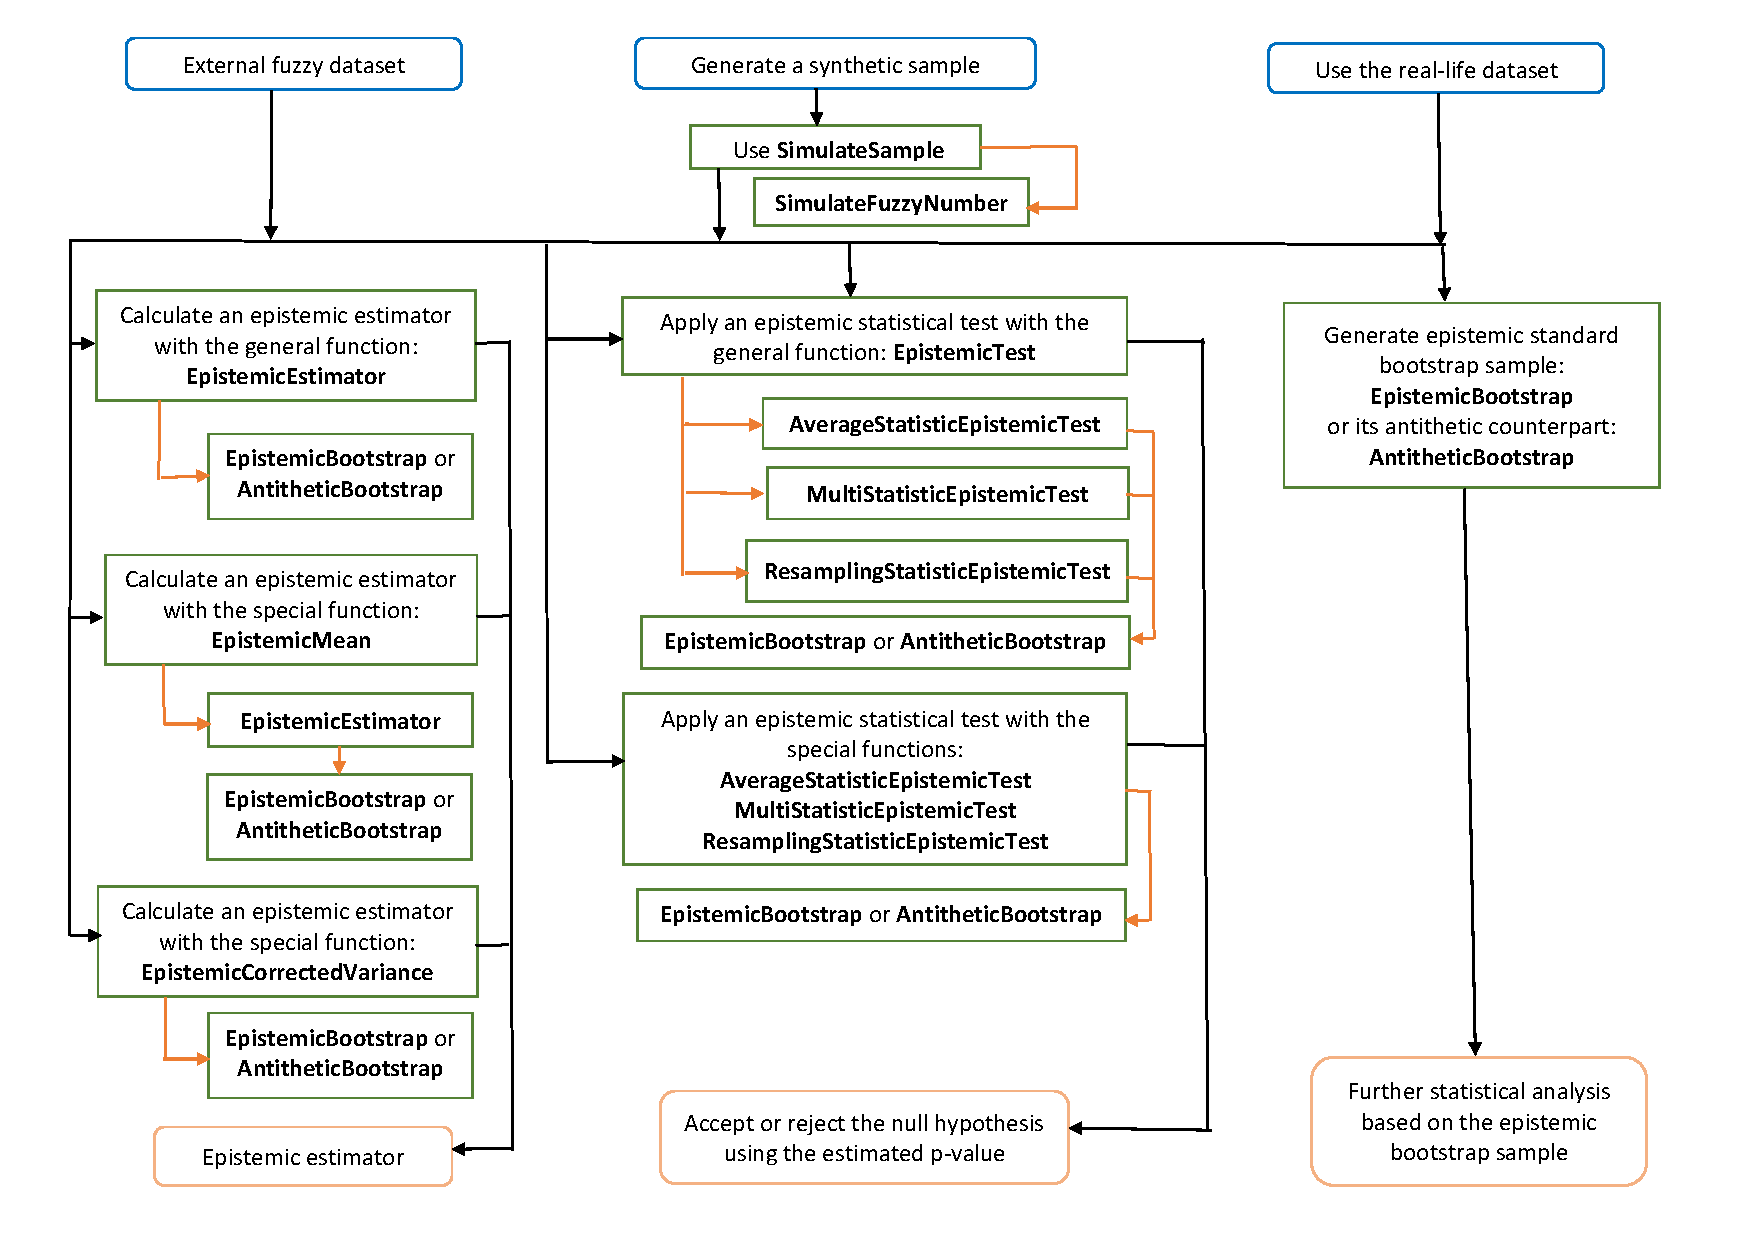
\includegraphics[scale=0.5]{flowchart3.pdf}
	\caption{General workflow for possible applications and invoking the functions from \pkg{FuzzySimRes} package.}
	\label{figflowchart1}
\end{figure}





%%%%%%%%%%%%%%%%%%%%%


\subsection{Generation of the initial sample}
\label{genofinsa}

In many cases, synthetic samples of predefined properties are necessary to analyze statistical methods numerically.
Two functions in \pkg{FuzzySimRes} allow the generation of random fuzzy variables.
The first one
\begin{example}
SimulateFuzzyNumber(originalPD,parOriginalPD,incrCorePD,
  parIncrCorePD,suppLeftPD,parSuppLeftPD,
  suppRightPD,parSuppRightPD,knotNumbers = 0,
  type = "trapezoidal",...)
\end{example}
is used to generate randomly a single TPFN (for \code{type = "trapezoidal"}), TRFN (\code{type = "triangular"}), or PLFN (\code{type = "PLFN"}, respectively).
All these types of FNs utilize the respective S4 objects from \pkg{FuzzyNumbers}.

To simulate a TPFN $\widetilde{X}$, five independent real-valued random variables are necessary: $X$ for its ``true value'' (i.e., its \textit{original}), $C^l, C^r$ -- the left and right increment of the core, $S^l$, $S^r$ -- the left and right increment of the support, respectively.
To generate these random variables the functions derived from \pkg{stats} \citep{RMan} with the respective parameters are used (see Table \ref{tab500}), e.g., to draw randomly the original $X$, the function \code{originalPD} with the parameters \code{parOriginalPD} should be applied.

\begin{table}[htbp]
\centering

\begin{tabular}{l|cc}
\hline 
 Random variable & Function & Parameters   \\ 
\hline
$X$ &  \code{originalPD} &  \code{parOriginalPD}  \\
$C^l, C^r$ & \code{incrCorePD} & \code{parIncrCorePD} \\
$S^l$ & \code{suppLeftPD} & \code{parSuppLeftPD} \\
$S^r$ & \code{suppRightPD} & \code{parSuppRightPD} \\
\hline

\end{tabular}
\caption{Random variables used to simulate a TPFN.}\label{tab500}
\end{table}

As a result we obtain a random TPFN given by $(X-C^l-S^l,X-C^l,X+C^r,X+C^r+S^r)$ (see also \cite{10.1007/978-3-031-08974-9_39} for the similar procedure).
Obviously, for a TRFN we have $C^l=C^r=0$ without using the respective parameters in \code{SimulateFuzzyNumber}.
In the case of a PLFN, the number of knots \code{knotNumbers} should be greater than zero, and then the specially truncated probability distributions for both arms of the support are applied.
The function \code{SimulateFuzzyNumber} returns both the generated FN (as \code{value} in the output list) and its random original $X$ (as \code{original}).


Let us initialize a random seed and generate a TPFN with the ``true origin'' described by the normal distribution with the expected value $\mu =0$ and standard deviation $\sigma=1$ (denoted by $N (\mu, \sigma)$), the increments of the core given by the uniform distribution on the interval $(0,0.6)$ (denoted by $U(0,0.6)$) and the increments of the support from $U(0,1)$:
\begin{example}
# seed PRNG
> set.seed(123456)

> SimulateFuzzyNumber(originalPD="rnorm",parOriginalPD=list(mean=0,sd=1),
+  incrCorePD="runif",parIncrCorePD=list(min=0,max=0.6),
+  suppLeftPD="runif",parSuppLeftPD=list(min=0,max=1),
+  suppRightPD="runif",parSuppRightPD=list(min=0,max=1),
+  type="trapezoidal")

$original
[1] 0.6857515

$value
Trapezoidal fuzzy number with:
   support=[-0.316967,1.10087],
      core=[0.480817,0.902528].
\end{example}


The second function generates a sample of \code{n} independent FNs similarly to \code{SimulateFuzzyNumber}:
\begin{example}
SimulateSample(n = 1,originalPD,parOriginalPD,incrCorePD,
  parIncrCorePD,suppLeftPD,parSuppLeftPD,
  suppRightPD,parSuppRightPD,knotNumbers = 0,
  type = "trapezoidal")
\end{example}
This function returns a list of simulated FNs together with a vector of their respective originals.
Let us generate 10 TPFNs given by the same distributions as in the previous example and print the second simulated value and its ``true origin'':
\begin{example}
# seed PRNG
> set.seed(123456)

> sample1 <- SimulateSample(n=10,originalPD="rnorm",
+  parOriginalPD=list(mean=0,sd=1),
+  incrCorePD="runif",parIncrCorePD=list(min=0,max=0.6),
+  suppLeftPD="runif",parSuppLeftPD=list(min=0,max=1),
+  suppRightPD="runif",parSuppRightPD=list(min=0,max=1),
+  type="trapezoidal")

> sample1$original[2]

[1] -1.301602

> sample1$value[2]

$X2
Trapezoidal fuzzy number with:
   support=[-1.937,-0.229014],
      core=[-1.40214,-0.822808].
      
> plot(sample1$value[[2]])
\end{example}

The obtained graph of this exemplary FN can be found in Fig. \ref{figFN1}.

\begin{figure}[htb]
  \centering
	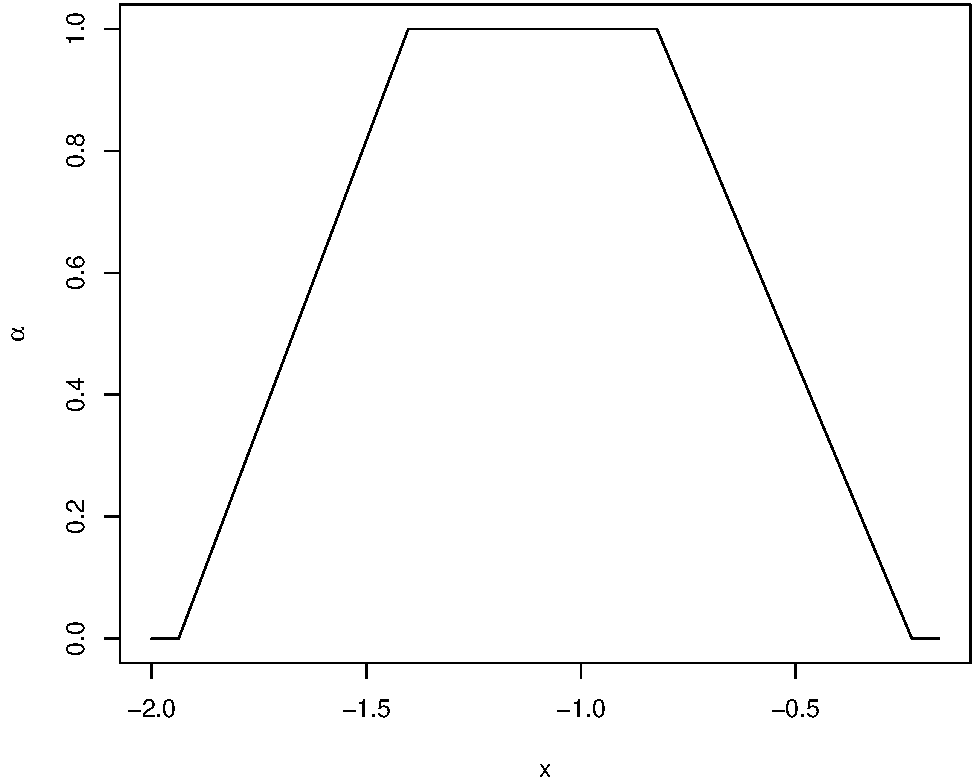
\includegraphics[scale=0.45]{fuzzy_number_rys1.pdf}
	\caption{Example of the generated TPFN.}
	\label{figFN1}
\end{figure}


%%%%%%%%%%%%%%%%%%%%%


\subsection{Epistemic bootstrap}

All of the functions  described in further sections use two main procedures related to the epistemic bootstrap  \citep{grzegorzewski2021,10.1007/978-3-031-08974-9_39,pgmr2022,PGMR2024AMS}.

The first one
\begin{example}
EpistemicBootstrap(fuzzySample, cutsNumber = 1,...)
\end{example}
applies the \textbf{standard epistemic bootstrap} (abbreviated as \emph{std}) to a single value or a whole list of FNs given by \code{fuzzySample}.
This procedure firstly generates uniformly a list of $\alpha$-cuts (their number is specified by \code{cutsNumber}). Then, it generates a sample from each of the input FNs, corresponding to the aforementioned list of the $\alpha$-cuts.
A final output is given as a real-valued matrix, with the number of rows that is equal to \code{cutsNumber}, and the number of columns designated by the initial sample size.
This way, we obtain $b$ real-valued bootstrap samples $\mathbb{X}^{*j} = \left ( X_1^{*j}, \ldots,  X_n^{*j} \right )$, based on the initial fuzzy sample $\tilde{\mathbb{X}} = ( \tilde{X}_1, \ldots,  \tilde{X}_n)$, where $j=1, \ldots,b$ and $b$ is equal to \code{cutsNumber}.

Let us apply the epistemic bootstrap with 3 $\alpha$-cuts for the previously generated \code{sample1}, and then show the output rounded to 4 decimal places:
\begin{example}
> set.seed(123456)

> epistemicOutput <- EpistemicBootstrap(sample1$value, cutsNumber = 3)

> round(epistemicOutput,digits = 4)

           X1      X2     X3     X4      X5     X6     X7      X8      X9    X10
0.7978 0.5323 -1.0784 0.6744 0.8553  0.9501 1.1755 0.6460 -0.5347 -0.0049 1.5937
0.7536 0.5253 -1.4512 1.4851 0.8546  0.9337 1.4773 0.6576 -0.3149 -0.0022 1.8909
0.3913 0.1991 -0.4767 1.1215 0.9443 -0.0089 0.8814 0.4538  0.0633 -0.9345 1.1242

\end{example}
The first column shows $\alpha$-cuts drawn randomly, while the rest columns contain values generated from each $\alpha$-cut.

The second function
\begin{example}
AntitheticBootstrap(fuzzySample, cutsNumber = 1,...)
\end{example}
applies the so-called \textbf{antithetic epistemic bootstrap} (denoted further on by \emph{anti}).
Instead of drawing a single value from the given $\alpha$-cut of each FN, we generate two values: one from this $\alpha$-cut and the other from $(1-\alpha)$-cut, and then we determine their average.
As indicated in \cite{10.1007/978-3-031-08974-9_39,pgmr2022}, the antithetic approach improves the quality of some statistical inference methods.
An example of how to use this function can be found in the supplementary file.

The epistemic bootstrap produces a real-valued sample based on the initial fuzzy values.
Therefore, it can be easily applied to estimate various statistical measures of the input values (like the mean) or to conduct many ``classical'' (i.e. real-valued) statistical tests.


%%%%%%%%%%%%%%%%%%%%%


\subsection{Estimation of parameters}


Estimation of basic population parameters (like the mean) is a fundamental task of most statistical inference problems. Given fuzzy data, we can easily adapt the epistemic bootstrap to estimate the quantities of interest (see  \citep{pgmr2022}).

A general function
\begin{example}
EpistemicEstimator(fuzzySample,estimator = "sd",cutsNumber = 1,bootstrapMethod = "std",
  trueValue = NA,...)
\end{example} 
can be used to determine the desired estimate from the \code{fuzzySample} of the specified function in \code{estimator}.
Both the classical epistemic approach (\code{bootstrapMethod = "std"}) and its antithetic counterpart (\code{bootstrapMethod = "anti"}) are  available.
Since the mean is the most used statistical parameter, it can be obtained using a special function
\begin{example}
EpistemicMean(fuzzySample,cutsNumber = 1,bootstrapMethod = "std",trueValue = NA,...)
\end{example}
instead of the general command.

Besides estimates, the standard error (SE) and the mean squared error (MSE) of the considered estimators are also calculated.
The SE is estimated (for $b >1$) using the formula
\begin{equation}
\label{frachetse}
	\widehat{\mathrm{SE}}=\sqrt{\frac{1}{b-1} \sum_{k=1}^{b} \left ( \hat{\theta} \left (\mathbb{X}^{*k} \right) - \bar{\hat{\theta}} \right )^2}  ,
\end{equation}
where $\hat{\theta} \left (\mathbb{X}^{*k} \right) $ is the estimator of $\theta$ based on the epistemic bootstrap sample for the $k$-th $\alpha$-cut, and $\bar{\hat{\theta}}$ is the overall mean for $\hat{\theta} \left (\mathbb{X}^{*1} \right),\ldots,\hat{\theta} \left (\mathbb{X}^{*b} \right)$.
If the true (but usually unknown) value of $\theta$ is set with \code{trueValue}, then the MSE is estimated by
\begin{equation}
\label{frachetmse}
	\widehat{\mathrm{MSE}}=\frac{1}{b} \sum_{k=1}^{b} \left ( \hat{\theta} \left (\mathbb{X}^{*k} \right) - \theta \right )^2 .
\end{equation}

Let us estimate the median and its SE for \code{sample1} using 100 $\alpha$-cuts and the classical epistemic bootstrap:
\begin{example}
> set.seed(56789)

> EpistemicEstimator(sample1$value, estimator = "median",cutsNumber = 100)

$value
[1] 0.6287525

$SE
[1] 0.1705336

$MSE
[1] NA
\end{example} 

To estimate the variance using bootstrap, instead of the classical well-known formula, its more sophisticated and specially corrected variant \citep{pgmr2022} can be used with the function
\begin{example}
EpistemicCorrectedVariance(fuzzySample,cutsNumber = 1,bootstrapMethod = "std",...)
\end{example}
As noted in \cite{pgmr2022}, this estimator can more closely approximate the desired value, e.g., we have
\begin{example}
> set.seed(56789)

> EpistemicCorrectedVariance(sample1$value, cutsNumber = 100$)

[1] 0.8729738
\end{example} 


%%%%%%%%%%%%%%%%%%%%%


\subsection{Statistical tests}


The real-valued samples generated by the epistemic bootstrap can be also used for hypothesis testing. 
However, given several bootstrap samples, one has to clarify how to merge the obtained test statistics or the p-values \citep{10.1007/978-3-031-08974-9_39}.
\pkg{FuzzySimRes} contains a general function 
\begin{example}
EpistemicTest(sample1, sample2, algorithm = "avs", ...)
\end{example}
that can be used to activate one of the specially tailored procedures.

By setting \code{algorithm = "avs"} the \textbf{averaging statistic} (abbreviated as \emph{avs}) is activated and the function
\begin{example}
AverageStatisticEpistemicTest(sample1,sample2,bootstrapMethod = "std",
  test = "ks.test",cutsNumber = 1,criticalValueFunction = "KSTestCriticalValue",...)
\end{example}
is used.
Similarly, by setting \code{algorithm = "ms"} the function
\begin{example}
MultiStatisticEpistemicTest(sample1,sample2,bootstrapMethod = "std",
  test = "ks.test",cutsNumber = 1,combineMethod = "simes",...)
\end{example}
and \textbf{multi-statistic} method (denoted by \emph{ms}) are applied.
Finally, for \code{algorithm = "res"} the \textbf{resampling} algorithm (abbreviated as \emph{res}) together with the function
\begin{example}
ResamplingStatisticEpistemicTest(sample1,sample2,bootstrapMethod = "std",
  test = "ks.test",cutsNumber = 1,K = 1,combineMethod = "simes",...)
\end{example}
run.
The above functions can be applied to both one-sample and two-sample statistical tests, where the relevant samples are entered as lists of fuzzy values. 
For the one-sample case, \code{sample2=NULL} should be set.

To use a statistical test, one has to specify the name of the respective function in \code{test} (e.g., \code{test="ks.test"} for \code{ks.test} from \pkg{stats} activates the Kolmogorov-Smirnov goodness-of-fit test, abbreviated further on as the KS test).
User-defined functions can be also used if they have at least one or two parameters (\code{x} for one- or \code{x,y} for two-sample case, namely) and return a list of at least two values (\code{statistic} for the output test statistic, and \code{p.value} for the calculated p-value).
In the case of the \emph{avs} approach, the additional parameter \code{criticalValueFunction} is required with the name of the function  calculating the p-value for a specified critical level of the considered test statistic.
For the KS test, such a procedure is given by \code{KSTestCriticalValue} available in \pkg{FuzzySimRes}.

To conduct the test, the classical epistemic approach (\code{bootstrapMethod = "std"}) or its antithetic version (\code{bootstrapMethod = "anti"}) can be applied.
The p-values (in the case of \emph{ms} or \emph{res} methods) are aggregated with the algorithm specified in \code{combineMethod}.
Besides \code{combineMethod="mean"}, i.e. the simple averaging of p-values, all other methods are as in the package \CRANpkg{palasso} \citep{palassoArt}.

Let us generate the second sample with the small shift in location and compare it with the previously generated \code{sample1} using the two-sample KS test with the \emph{anti} and \emph{ms} approaches for 100 $\alpha$-cuts:
\begin{example}
> set.seed(56789)

> sample2 <- SimulateSample(n=10,originalPD="rnorm",
+  parOriginalPD=list(mean=0.5,sd=1),
+  incrCorePD="runif",parIncrCorePD=list(min=0,max=0.6),
+  suppLeftPD="runif",parSuppLeftPD=list(min=0,max=1),
+  suppRightPD="runif", parSuppRightPD=list(min=0,max=1),
+  type="trapezoidal")

> EpistemicTest(sample1$value,sample2$value,algorithm = "ms",
+  bootstrapMethod="anti",cutsNumber=100)

[1] 0.1873127
\end{example}
An example of the one-sample KS test can be found in the supplementary file. 


%%%%%%%%%%%%%%%%%%%%%


\subsection{Real-life dataset}


\pkg{FuzzySimRes} provides a fuzzy epistemic dataset \code{controlChartData} concerning electronic circuit thickness, which is one of the most important quality characteristics in the production of the electronic boards for vacuum cleaners (see \cite{FARAZ20102684} for the relevant source).
This dataset is given as a list of 90 TRFNs and contains 30 samples, each of size three.
Every observation has its own label \code{X.y.z}, where \code{y} is a sample number, and \code{z} stands for the element number in a sample, e.g.
\begin{example}
> controlChartData$X.1.2$

Trapezoidal fuzzy number with:
   support=[70.19,74.15],
      core=[71.4,71.4].
\end{example}
is the second value in the first sample.
 

%%%%%%%%%%%%%%%%%%%%%


\section{Statistical applications with the package}


As it was mentioned, the epistemic bootstrap provides real-valued samples generated from the initial fuzzy sample. It enables us to apply many classical statistical methods instead of using procedures specifically designed for fuzzy data (usually underdeveloped in the R environment).
In the following, we present some statistical applications of such approaches for both synthetic and real-life datasets.

In the first case, using \code{SimulateSample}, the respective samples are generated from the probability distributions described in Table \ref{tab100}.
Available TPFNs are grouped by their types, wherein the normal distribution with the mean $\mu$ and standard deviation $\sigma$ is denoted by $\mathrm{N}(\mu,\sigma)$, the uniform distribution on the interval $(a,b)$ -- by $\mathrm{U}(a,b)$, the exponential distribution with the parameter $\lambda$ -- by $\mathrm{Exp}(\lambda)$, the Weibull distribution with the shape $k$ and scale $\lambda$ parameters -- by $\mathrm{Weib} (k,\lambda)$, and the Gamma distribution with the shape $\alpha$ and rate $\beta$ parameters  -- by $\Gamma (\alpha,\beta)$, respectively.
In the case of the real-life dataset, the data \code{controlChartData} embedded in \pkg{FuzzySimRes} is applied.

In the following, only some of the results are presented in the tables and graphs to reduce the overall length of the paper.
All of the outputs can be found in the supplementary script file.

\begin{table}[htbp]
\centering

\begin{tabular}{l|cccc}
\hline 
 Type & $X$ & $C^l,\, C^r$ & $S^l$ &  $ S^r$   \\ 
\hline
$\mathbb{F}_{(\mathrm{N,U,U,U})}$ & $\mathrm{N}(0,1)$ & $\mathrm{U}(0,0.6)$ &  $\mathrm{U}(0,1)$ &  $\mathrm{U}(0,1)$  \\
$\mathbb{F}_{(\mathrm{Weib,Exp,Exp,Exp})}$ & $\mathrm{Weib} (2,1)$ &  $\mathrm{Exp}(5)$ & $\mathrm{Exp}(5)$ & $\mathrm{Exp}(4)$\\
$\mathbb{F}_{(\Gamma,\mathrm{U,U,U})}$ & $\Gamma (2,2)$ & $\mathrm{U}(0,0.6)$ &  $\mathrm{U}(0,0.8)$ &  $\mathrm{U}(0,0.8)$  \\
\hline

\end{tabular}
\caption{Scenarios for simulating fuzzy random variables.}\label{tab100}
\end{table}


%%%%%%%%%%%%%%%%%%%%%


\subsection{Comparison of estimators}

We start with a comparison of some estimators of the mean, variance, and median for both epistemic approaches, i.e., the \emph{std} and \emph{anti}.
For all types of the TPFNs mentioned in Table \ref{tab100}, the function \code{EpistemicEstimator} was applied with $b=100$ $\alpha$-cuts.
To limit the randomness impact, each numerical experiment was repeated $m=1000$ times.
Both small ($n=10$) and moderate ($n=100$) samples were considered.

Since the function \code{SimulateSample}  produces also the ``true values'' of the fuzzy samples (i.e., their originals), it gives an opportunity (quite exceptional in real-life applications) to compare the epistemic bootstrap estimators based on fuzzy samples with the results related to these originals.
Then, we can calculate the respective error -- \textbf{Originals Absolute Error} (abbreviated as OAE) -- that measures the absolute difference between the epistemic bootstrap estimator $\hat{\theta}^*_{j}$ based on the $j$-th synthetic sample and its counterpart $\hat{\theta}^o_{j}$ obtained from the originals for this $j$-th sample, i.e.,
\begin{equation}
    \text{OAE} = \frac{1}{m}\sum_{j=1}^{m} \left | \hat{\theta}^*_{j} - \hat{\theta}^o_{j} \right | ,
\end{equation}
where $m$ is the number of simulations.

In general, it seems that the \emph{anti} approach gives better results -- the resulting estimates are closer to their ``true'' values and the respective errors are lower (see Table \ref{tab200} and the supplementary file).
To facilitate the understanding of Table \ref{tab200}, the best outputs (i.e., the estimators that are the closest to the respective true values of the parameters, and the lowest errors in each case) are given in boldface there.
Of course, the answers may vary for the different error measures (e.g., sometimes the OAE is slightly lower for the \emph{std} approach).
However, the \emph{anti} method clearly provides the significant improvement measured with the SE, slightly less important (but still visible) in the case of the MSE.
Taking into account the low additional numerical burden of this approach when it is compared with the \emph{std} method (i.e. generation of two values: from the $\alpha$-cut and its $(1-\alpha)$ counterpart instead of only a single drawing), the \emph{anti} algorithm should be recommended to users.
The above-mentioned conclusions are similar to the ones discussed in \cite{grzegorzewski2021,pgmr2022}.


\begin{table}[htbp]
\centering
\begin{tabular}{l|cc|cc|cc}
\hline
 & \multicolumn{2}{c|}{Mean} & \multicolumn{2}{c|}{Variance} & \multicolumn{2}{c}{Median} \\
  \hline
 & std & anti & std & anti & std & anti \\ 
  \hline
  
\multicolumn{7}{l}{$\mathbb{F}_{(\mathrm{N,U,U,U})}, n=10$} \\

  \hline
Value & -0.0055 & \textbf{-0.0053} & 1.1476 & \textbf{1.0854} & \textbf{-0.0034} & -0.0038 \\ 
  SE & 0.1089 & \textbf{0.0760} & 0.2424 & \textbf{0.1595} & 0.1797 & \textbf{0.1347} \\ 
  MSE & 0.1145 & \textbf{0.1078} & 0.3469 & \textbf{0.2972} & 0.1602 & \textbf{0.1522} \\ 
  OAE & 0.0407 & \textbf{0.0405} & 0.1555 & \textbf{0.1105} & 0.0874 & \textbf{0.0819} \\
   \hline
  
\multicolumn{7}{l}{$\mathbb{F}_{(\mathrm{N,U,U,U})}, n=100$} \\
  \hline
Value & 0.0016 & 0.0016 & 1.1472 & \textbf{1.0850} & \textbf{0.0004} & 0.0006 \\ 
  SE & 0.0345 & \textbf{0.0242} & 0.0999 & \textbf{0.0498} & 0.0705 & \textbf{0.0573} \\ 
  MSE & 0.0115 & \textbf{0.0110} & 0.0526 & \textbf{0.0305} & 0.0179 & \textbf{0.0168} \\ 
  OAE & 0.0135 & \textbf{0.0134} & 0.1480 & \textbf{0.0860} & 0.0405 & \textbf{0.0375} \\ 
  \hline
\multicolumn{7}{l}{$\mathbb{F}_{(\mathrm{Weib,Exp,Exp,Exp})}, n=10$} \\
  \hline
  
Value & 0.8917 & \textbf{0.8912} & 0.2884 & \textbf{0.2671} & 0.8536 & \textbf{0.8517} \\ 
  SE & 0.0636 & \textbf{0.0440} & 0.0728 & \textbf{0.0478} & 0.0941 & \textbf{0.0706} \\ 
  MSE & 0.0272 & \textbf{0.0251} & 0.0287 & \textbf{0.0222} & 0.0398 & \textbf{0.0378} \\ 
  OAE & \textbf{0.0409} & 0.0412 & 0.0716 & \textbf{0.0553} & \textbf{0.0609} & 0.0621 \\ 

  \hline
\multicolumn{7}{l}{$\mathbb{F}_{(\mathrm{Weib,Exp,Exp,Exp})}, n=100$} \\
  \hline

Value & \textbf{0.8864} & 0.8865 & 0.2828 & \textbf{0.2614} & 0.8417 & \textbf{0.8387} \\ 
  SE & 0.0203 & \textbf{0.0141} & 0.0295 & \textbf{0.0152} & 0.0359 & \textbf{0.0290} \\ 
  MSE & 0.0029 & \textbf{0.0027} & 0.0068 & \textbf{0.0037} & 0.0044 & \textbf{0.0041} \\ 
  OAE & 0.0127 & 0.0127 & 0.0676 & \textbf{0.0462} & 0.0252 & \textbf{0.0247} \\ 

   \hline
\end{tabular}
\caption{Numerical comparison of the estimators (for the mean, variance, and median) and their errors (the standard error -- SE, the mean squared error -- MSE, and the originals absolute error -- OAE) based on the epistemic bootstrap (the standard -- std,  and the antithetic epistemic bootstrap -- anti).}\label{tab200}
\end{table}


%%%%%%%%%%%%%%%%%%%%%


\subsection{Detection of the difference in location}


Then, we conducted the power analysis for the two-sample KS test taking into account all the considered epistemic bootstrap approaches.
Two independent samples corresponding to the types of the TPFNs from Table \ref{tab100} were generated and the deterministic shift was added to the second sample.
As previously, both the small ($n=10$) and moderate ($n=100$) samples were considered, and each numerical experiment was repeated $m=1000$ times.
Besides the estimation of the null hypothesis rejection percentage for the significance level $\alpha =0.05$, the p-values for the increasing shift were also obtained and aggregated by simple averaging.

Using \code{SimulateSample} which delivers the originals of the simulated fuzzy sample, we can compare the results of the epistemic bootstrap tests with their ``crisp'' counterpart, so the results of the classical two-sample KS test serve us as a benchmark.
We can see that the estimated p-values (see Fig.~\ref{figN100pvalue1}) and power curves (see Fig. \ref{figN100power1}) for the moderate sample of TPFNs described by $\mathbb{F}_{(\mathrm{N,U,U,U})}$ are very close to their respective benchmarks, especially for the shift larger than 0.75.
To visualize the results better, the differences in p-values and power curves between the epistemic bootstrap approaches and the classical KS test were also calculated (see Fig. \ref{figN100pvalue2} and \ref{figN100power2}, respectively).
   

\begin{figure}[htb]
  \centering
	\begin{minipage}[t]{0.42\linewidth}
	\vspace{0pt}
	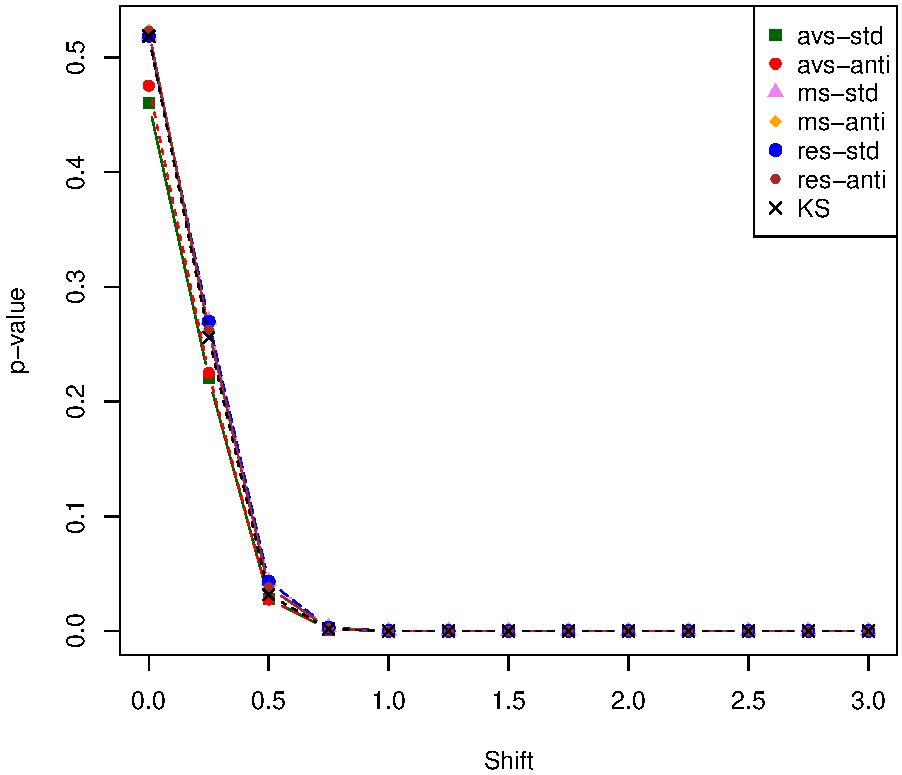
\includegraphics[scale=0.42]{pvalue_N100_rys01.pdf}
	\caption{Estimated p-values of the two-sample epistemic and ``crisp'' KS tests for $\mathbb{F}_{(\mathrm{N,U,U,U})}, n=100$, and shift in location.}
	\label{figN100pvalue1}
	\end{minipage}  
\hfill
\begin{minipage}[t]{0.45\linewidth}
\vspace{0pt}
	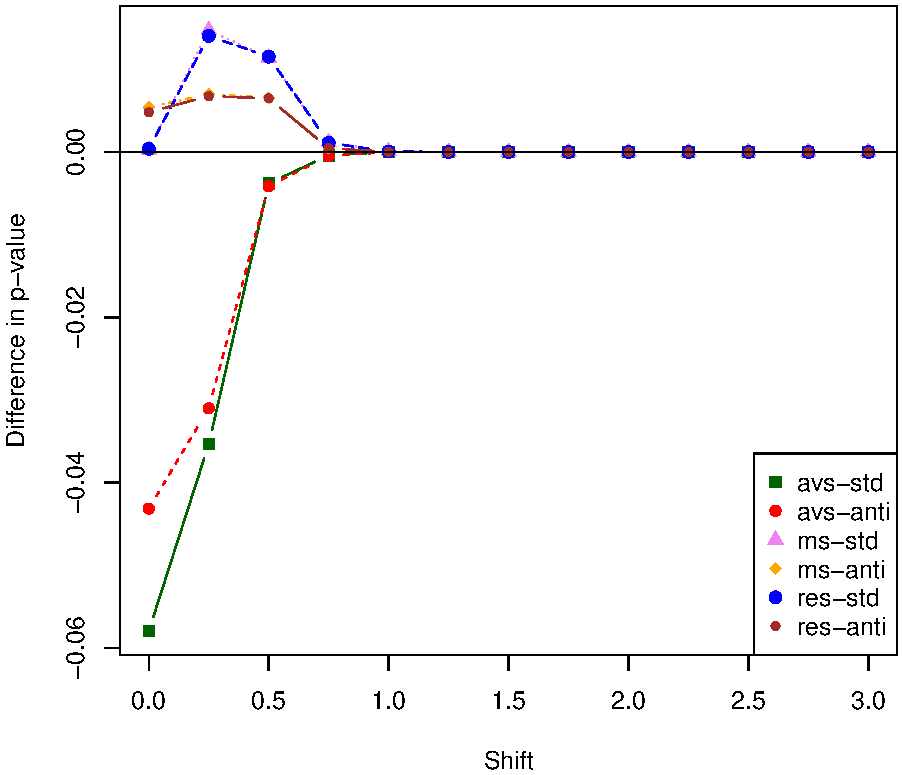
\includegraphics[scale=0.42]{diff_pvalue_N100_rys01.pdf}
	\caption{Differences in estimated p-values between the two-sample epistemic and ``crisp'' KS tests for $\mathbb{F}_{(\mathrm{N,U,U,U})}, n=100$, and shift in location.}
	\label{figN100pvalue2}
	\end{minipage}  
\end{figure}


\begin{figure}[htb]
  \centering
	\begin{minipage}[t]{0.45\linewidth}
	\vspace{0pt}
	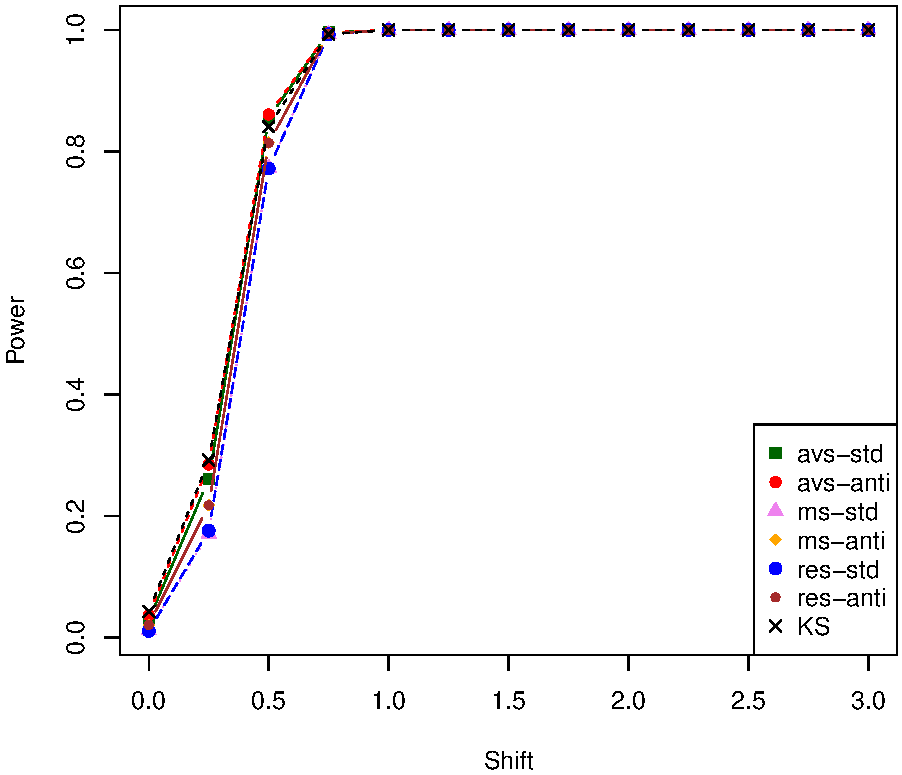
\includegraphics[scale=0.42]{power_N100_rys01.pdf}
	\caption{Power curves of the two-sample epistemic and ``crisp'' KS tests for $\mathbb{F}_{(\mathrm{N,U,U,U})}, n=100$, and shift in location.}
	\label{figN100power1}
	\end{minipage}  
\hfill
\begin{minipage}[t]{0.45\linewidth}
\vspace{0pt}
	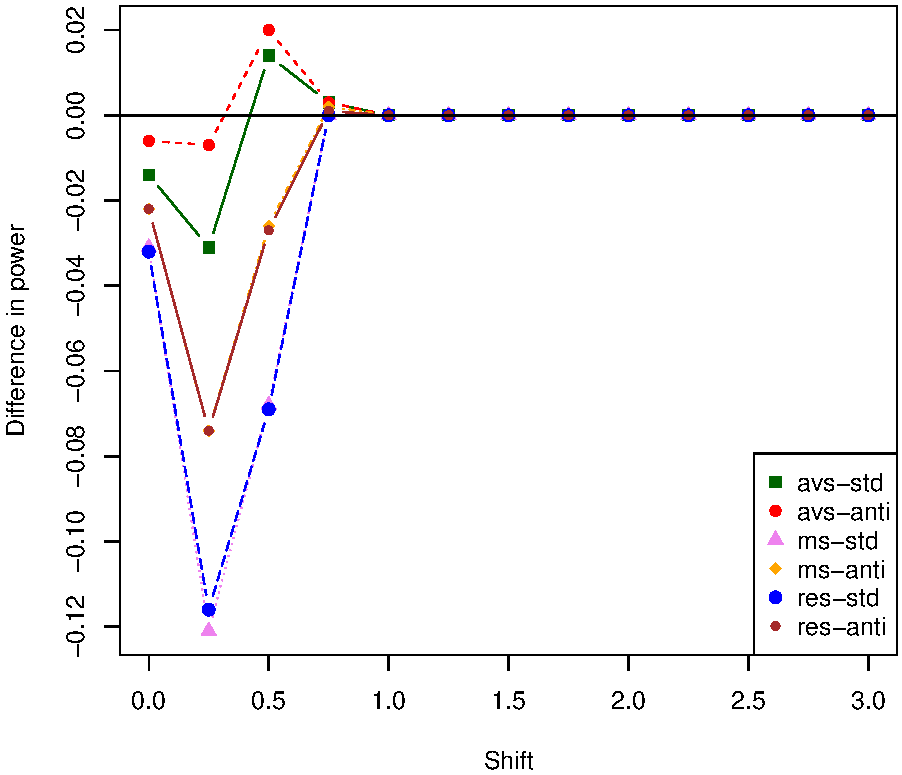
\includegraphics[scale=0.42]{diff_power_N100_rys01.pdf}
	\caption{Differences in power curves between the two-sample epistemic and ``crisp'' KS tests for $\mathbb{F}_{(\mathrm{N,U,U,U})}, n=100$, and shift in location.}
	\label{figN100power2}
	\end{minipage}  
\end{figure}


In general, the estimation error for p-values is lower when the \emph{ms} or \emph{res} approaches are used (especially when they are combined with the \emph{anti} method), and the power curves are closer to the respective benchmarks for the \emph{avs} and \emph{ms} algorithms (the \emph{anti} method has also a beneficial effect).
Additional examples can be found in the supplementary file and \cite{10.1007/978-3-031-08974-9_39}.


%%%%%%%%%%%%%%%%%%%%%


\subsection{Detection of the difference in scale}

Next, we conducted the power study of tests to detect the difference in dispersion.
This case was modeled by gradually increasing the standard deviation of the second sample when the first one is simulated according to $\mathbb{F}_{(\mathrm{N,U,U,U})}$ type.

As previously, the p-values and power curves (see Fig. \ref{figN100pvaluesd1} and \ref{figN100powersd1}) were estimated for the moderate sample and the respective simulation parameters: $m=1000$, $\alpha=0.05$, and $b=100$.
A comparison of the epistemic bootstrap approaches and our benchmark (i.e., the two-sample ``crisp'' KS test) was also done (see Fig. \ref{figN100pvaluesd2} and \ref{figN100powersd2}, respectively).
It seems that the estimation error of p-values is lower for the \emph{ms} or \emph{res} approach and the power curves are closer to the respective results of the ``crisp'' KS test for the \emph{avs} and \emph{ms} algorithms. Thus, the \emph{anti} method again improves the results.

An additional example for the small sample is provided in the supplementary file.


\begin{figure}[htb]
  \centering
	\begin{minipage}[t]{0.45\linewidth}
	\vspace{0pt}
	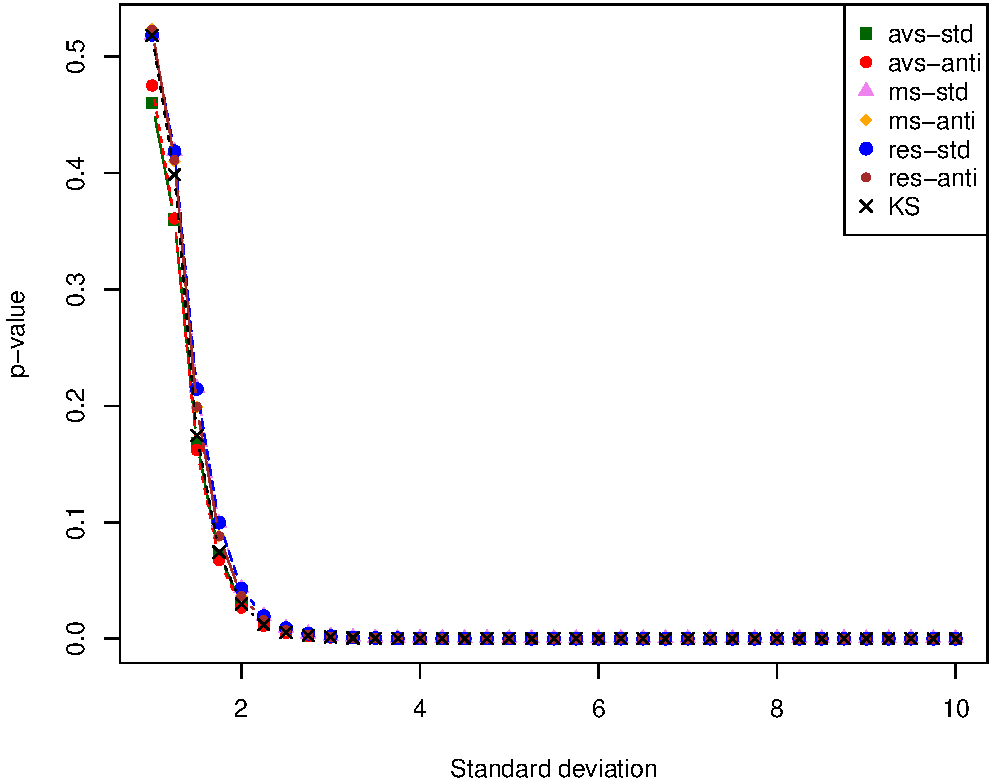
\includegraphics[scale=0.4]{pvalue_sd_N100_rys01.pdf}
	\caption{Estimated p-values of the two-sample epistemic and ``crisp'' KS tests for $\mathbb{F}_{(\mathrm{N,U,U,U})}, n=100$, difference in scale.}
	\label{figN100pvaluesd1}
	\end{minipage}  
\hfill
\begin{minipage}[t]{0.45\linewidth}
\vspace{0pt}
	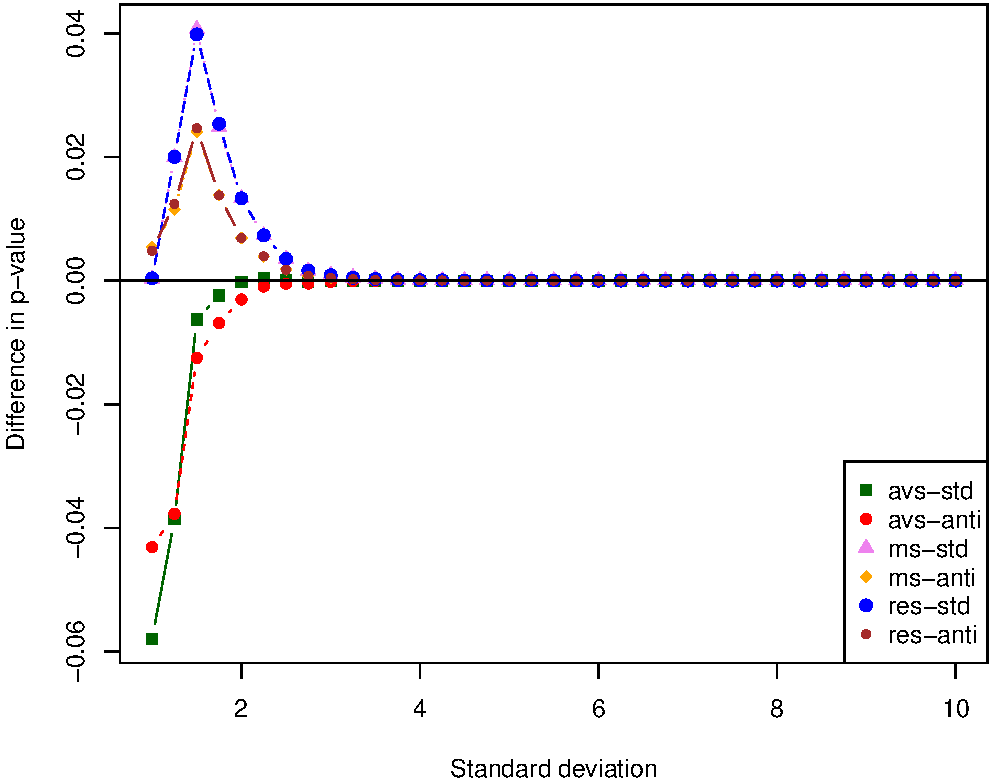
\includegraphics[scale=0.38]{diff_pvalue_sd_N100_rys01.pdf}
	\caption{Differences in estimated p-values between the two-sample epistemic and ``crisp'' KS tests for $\mathbb{F}_{(\mathrm{N,U,U,U})}, n=100$, difference in scale.}
	\label{figN100pvaluesd2}
	\end{minipage}  
\end{figure}



\begin{figure}[htb]
  \centering
	\begin{minipage}[t]{0.45\linewidth}
	\vspace{0pt}
	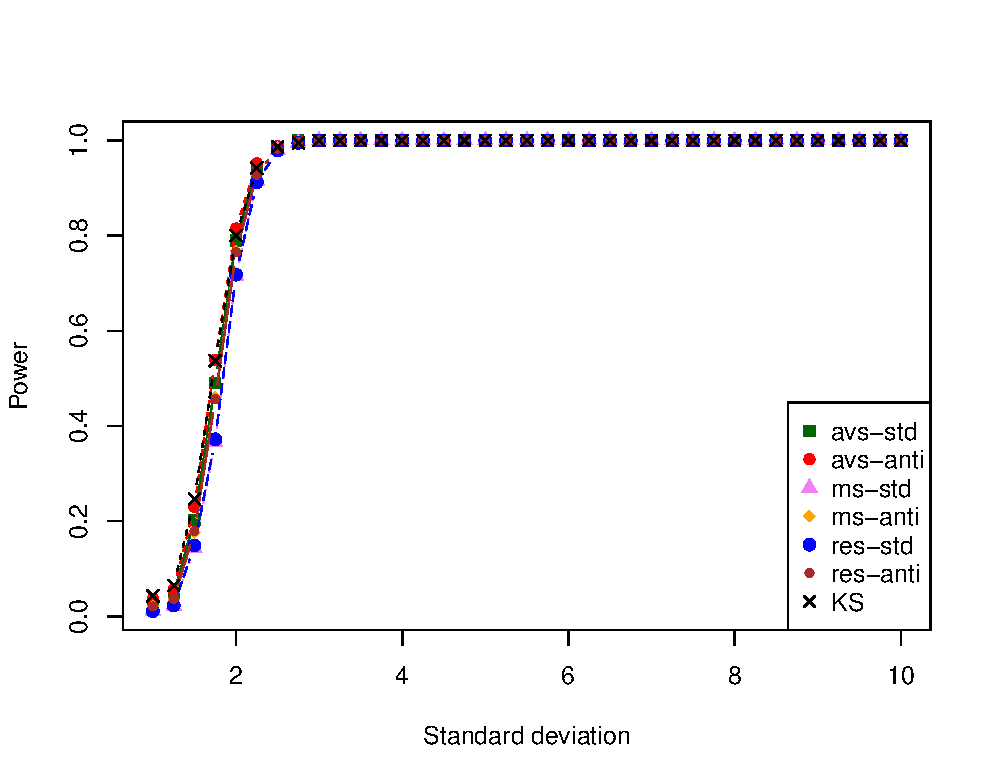
\includegraphics[scale=0.4]{power_sd_N100_rys01.pdf}
	\caption{Power curves of the two-sample epistemic and ``crisp'' KS tests for $\mathbb{F}_{(\mathrm{N,U,U,U})}, n=100$, difference in scale.}
	\label{figN100powersd1}
	\end{minipage}  
\hfill
\begin{minipage}[t]{0.45\linewidth}
\vspace{0pt}
	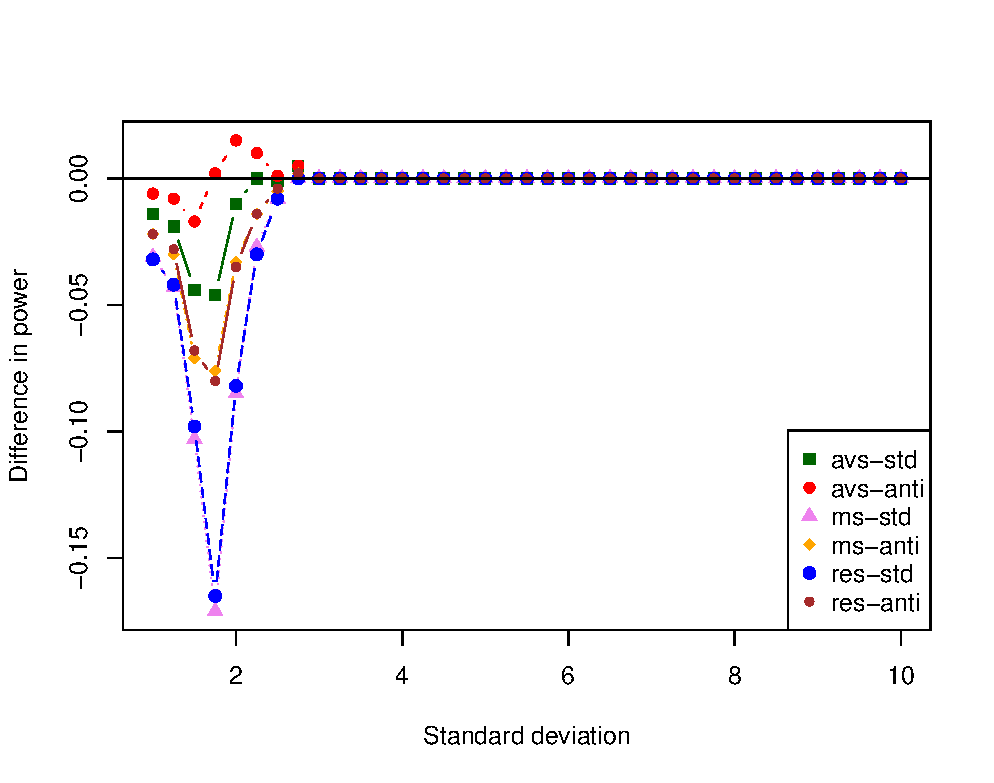
\includegraphics[scale=0.4]{diff_power_sd_N100_rys01.pdf}
	\caption{Differences in power curves between the two-sample epistemic and ``crisp'' KS tests for $\mathbb{F}_{(\mathrm{N,U,U,U})}, n=100$, difference in scale.}
	\label{figN100powersd2}
	\end{minipage}  
\end{figure}


%%%%%%%%%%%%%%%%%%%%%


\subsection{Goodness-of-fit test in quality control}


Finally, we applied the KS two-sample test for the manufacturing data embedded in \pkg{FuzzySimRes}.
These fuzzy data can be used to build the respective control charts to check the behavior of the underlying process \citep{FARAZ20102684}.
But in our experiment, the sample was divided randomly into two parts to check if they came from the same distribution (so they were ``not statistically different'').

\begin{example}
> set.seed(5678)
> randomSetsCCD <- sample(length(controlChartData),length(controlChartData)/2)

> EpistemicTest(controlChartData[randomSetsCCD],controlChartData[-randomSetsCCD],
+  algorithm="avs",cutsNumber=1000)

[1] 0.3319477

> EpistemicTest(controlChartData[randomSetsCCD],controlChartData[-randomSetsCCD],
+  algorithm="ms",combineMethod="mean",cutsNumber=1000)

[1] 0.433548

> EpistemicTest(controlChartData[randomSetsCCD],controlChartData[-randomSetsCCD],
+  algorithm="res",combineMethod="mean",cutsNumber=1000,K=200)

[1] 0.4616578
\end{example}

As we can see, all of the considered algorithms do not reject the null hypothesis for the KS test, even for high significance levels.
These results are consistent with the findings in \cite{FARAZ20102684}.
Moreover, as \cite{PGMR2024AMS} described, the epistemic KS test clearly indicates the issues caused by the troublesome 21st subsample.
It makes the process out of control and results in the lower p-values in the goodness-of-fit tests.


%%%%%%%%%%%%%%%%%%%%%


\section{Conclusions}


\pkg{FuzzyResampling} package delivers resampling methods developed to overcome some shortcomings of the classical Efron's bootstrap in the fuzzy environment (see also \cite{fuzzyResamplingArt}).
However, this package was intended for the ontic fuzzy data.

Meanwhile, \pkg{FuzzySimRes} is a package that has a completely new purpose. The proposed epistemic bootstrap methods allow the generation of real-valued samples from the epistemic fuzzy data, which can then be directly utilized as input values for the various classical statistical procedures (like estimators, tests, etc.). It seems that the proposed methods combined with some well-known statistical techniques can be competitive with available fuzzy procedures which are not too popular among practitioners. Moreover, as was shown in the respective examples, the results of the suggested approaches implemented to imprecise data are comparable with their counterparts -- the benchmarks related to the real-valued originals of the fuzzy perceptions.

Of course, further investigations on epistemic bootstrap are still required. They can be aimed both at new resampling epistemic procedures and their applications in statistical inference and machine learning.


%%%%%%%%%%%%%%%%%%%%%


\bibliography{epistemicznyBootstrap}

  
%%%%%%%%%%%%%%%%%%%%%
  
  \address{Maciej Romaniuk\\
    Systems Research Institute Polish Academy of Sciences\\
    Newelska 6, 01-447 Warsaw\\
    Poland\\
	WIT Academy\\
    Newelska 6, 01-447 Warsaw\\
    Poland\\
    (0000-0001-9649-396X)\\
    \email{mroman@ibspan.waw.pl}}
  
  \address{Przemys{\l}aw Grzegorzewski\\
    Faculty of Mathematics and Information Science, Warsaw University of Technology \\
    Koszykowa 75, 00-662 Warsaw\\
    Poland\\
    Systems Research Institute Polish Academy of Sciences\\
    Newelska 6, 01-447 Warsaw\\
    Poland\\
    (0000-0002-5191-4123)\\
    \email{przemyslaw.grzegorzewski@pw.edu.pl}}
    
   \address{Abbas Parchami\\
       Department of Statistics, Faculty of Mathematics and Computer\\
       Shahid Bahonar University of Kerman, Kerman\\
       Iran\\
       (0000-0002-0593-7324)\\
       \email{parchami@uk.ac.ir}}
